\documentclass[a4paper,twoside]{article}


\usepackage{apalike}
\usepackage{SCITEPRESS}
\usepackage{amssymb}
\usepackage{amstext}
\usepackage{amsmath}
\usepackage{amsthm}

\usepackage{multicol}
\usepackage[small]{caption}

\usepackage{tikz}



\begin{document}


%%%%%%%%%%%%%%%%%%%%%%%%%%%%%%%%%%%%%%%%%%%%%%%%%%%%%%%%%%%%%%%%%%%%%%%%%%%%%%%%
%%%                               80 COLONNES                                %%%
%%%%%%%%%%%%%%%%%%%%%%%%%%%%%%%%%%%%%%%%%%%%%%%%%%%%%%%%%%%%%%%%%%%%%%%%%%%%%%%%


\title{RIOT OS Paves the Way for Implementation of High-Performance
       MAC Protocols}


%\author{
%\authorname{K\'evin Roussel, Ye-Qiong Song and Olivier Zendra}
%\affiliation{LORIA/INRIA Nancy Grand-Est,\\
%             Universit\'e de Lorraine,\\
%             615, rue du Jardin Botanique,\\
%             54600 Villers-L\`es-Nancy, France}
%\email{\{Kevin.Roussel,Ye-Qiong.Song,Olivier.Zendra\}@inria.fr}
%}


\keywords{Real-Time, Wireless Sensor Networks, Internet of Things,
          MAC protocols, RIOT OS}


\abstract{Implementing new, high-performance MAC protocols requires
real-time features, to be able to synchronize correctly between different
unrelated devices. Such features are highly desirable for operating
wireless sensor networks (WSN) that are designed to be part of the Internet
of Things (IoT). Unfortunately, the existing operating systems used in this
domain cannot provide such features. On the other hand, ``bare-metal''
development sacrifices portability, as well as the multitasking abilities
needed to develop the rich applications that are useful in the domain of
the Internet of Things.\\
We describe in this paper the development of a port of RIOT OS
on the MSP430 microcontroller architecture widely used in IoT-enabled motes.
RIOT OS offers rich and advanced  real-time features, especially the
simultaneous use of as many hardware timers as the underlying platform (MCU)
can offer. We then demonstrate the power of these features by providing
a new implementation of S-CoSenS, an efficient MAC protocol that uses
very low processing power and energy.}


\onecolumn \maketitle \normalsize \vfill

%%%%%%%%%%%%%%%%%%%%%%%%%%%%%%%%%%%%%%%%%%%%%%%%%%%%%%%%%%%%%%%%%%%%%%%%%%%%%

\section{\uppercase{Introduction}}

When programming the small devices that constitutes the nodes of
the Internet of Things (IoT), one has to adapt to the limitations of
these devices.

Apart from their very limited processing power (especially compared to
the current personal computers, and even mobile devices like smartphones
and tablets), the main specificity of the devices is that they are operated
on small batteries (e.g.: AAA or button cells).

Thus, one of the main challenges with these motes is the need to reduce
as much as possible their energy consumption. We want their batteries to last
as long as possible, for economical but also practical reasons: it may be
difficult---even almost impossible---to change the batteries of some of these
motes, because of their locations (e.g.: on top of buildings, under roads,
etc.)

IoT motes are usually very compact devices: they are usually built around
a central integrated chip that contains the main processing unit and several
basic peripherals (such as timers, A/D and D/A converters, I/O controllers...)
called microcontroller units or MCUs. Apart from the MCU, a mote generally
only contains some ``physical-world'' sensors and a radio transceiver for
networking. The main radio communication protocol currently used in the IoT
field is IEEE 802.15.4. Some MCUs do integrate a 802.15.4 transceiver on-chip.

Among the various components that constitute a mote, the most power-consuming
block is the radio transceiver. Consequently, to reduce the power consumption
of IoT motes, a first key point is to use the radio transceiver only when
needed, keeping it powered-off as much as possible. The software element
responsible to control the radio transceiver in an adequate manner is
the \emph{MAC~/ RDC (Media Access Control \& Radio Duty Cycle)}
layer of the network stack.

A efficient power-saving strategy for IoT motes thus relies on finding the
better trade-off between minimizing the radio duty cycle while keeping
networking efficiency at the highest possible level. This is achieved
by developing new, ``intelligent'' MAC~/ RDC protocols.

To implement new, high-performance MAC~/ RDC protocols, one needs to be
able to react to events with good reactivity (lowest latency possible) and
flexibility. These protocols rely on precise timing to ensure efficient
synchronization between the different motes and other radio-networked
devices of a \emph{Personal Area Network (PAN)}, thus allowing
to turn on the radio transceivers \emph{only} when needed.

At the system level, being able to follow such accurate timings means having
very efficient interruption management, and the extensive use of hardware
timers, that are the most precise timing source available.

The second most power-consuming element in a mote, after the radio
transceiver, is the MCU itself: every current MCU offers ``low-power modes'',
that consist in disabling the various hardware blocks, beginning with the CPU
core. The main way to minimize energy consumption with a MCU is thus
to disable its features as much as possible, only using them when needed:
that effectively means putting the whole MCU to sleep as much as possible.

Like for the radio transceiver, using the MCU efficiently while keeping
the system efficient and reactive means optimal use of interruptions,
and hardware timers for synchronization.

Thus, in both cases, we need to optimally use interruptions, and hardware
timers. Being able to use them both efficiently without too much hassle
implies the use of a specialized operating system (OS), especially
to easily benefit from multitasking abilities. That's what we will
discuss in this paper.

%%%%%%%%%%%%%%%%%%%%%%%%%%%%%%%%%%%%%%%%%%%%%%%%%%%%%%%%%%%%%%%%%%%%%%%%%%%%%

\section{\uppercase{Problem statement}}

Specialized OSes for the resource-constrained devices that constitute
wireless sensor networks have been designed, published, and made available
for quite sa long time.


The first widely used system in this domain was \emph{TinyOS} \cite{TinyOS}.
It is an open-source OS, whose first stable release (1.0) was published in
september 2002. It is very lightweight, and as such well adapted to limited
devices like WSN motes.  It has brought many advances in this domain, like
the ability to use Internet Protocol (IP) and routing (RPL) on 802.15.4
networks, including the latest IPv6 version, and to simulate networks
of TinyOS motes via TOSSIM \cite{TOSSIM}.

Its main drawback is that one needs to learn a specific language---named
nesC---to be able to efficiently work within it. This language is quite
different from standard C and other common imperative programming languages,
and as such can be difficult to master.

The presence of that specific language is no coincidence: TinyOS is built
on its own specific paradigms: it has an unique stack, from which the
different components of the OS are called as statically linked callbacks.
This makes the programming of applications complex, especially for
decomposing into various ``tasks''. The multitasking part is also
quite limited: tasks are run in a fixed, queue-like order. Finally,
TinyOS needs a custom GNU-based toolchain to be built.

All of these limitations, plus a relatively slow development pace (last
stable version dates back to august 2012) have harmed its adoption,
and it is not the mainly used OS of the domain anymore.


The current reference OS in the domain of WSN and IoT is \emph{Contiki}
\cite{ContikiOS}. It's also an open-source OS, which was first released
in 2002. It is also at the origin of many assets: we can cite, among others,
the uIP Embedded TCP/IP Stack \cite{uip}, that has been extended to uIPv6,
the low-power Rime network stack \cite{Rime}, or the Cooja advanced network
simulator \cite{Cooja}.

While a bit more resource-requiring than TinyOS, Contiki is also very
lightweight and well adapted to motes. Its greatest advantage over TinyOS
is that it is based on standard, well-known OS paradigms, and coded
in standard C language, which makes it relatively easy to learn and program.
It offers an event-based kernel, implemented using cooperative multithreading,
and (as we said before) a complete network stack. All of these features and
advantages have made Contiki widespread: as we said before, it is currently
the reference OS when it comes to WSN.

Contiki developers also have made advances in the MAC/RDC domain: many
of them have been implemented as part of the Contiki network stack, and
a specifically developed, ContikiMAC, has been published in 2011
\cite{ContikiMAC} and implemented into Contiki as the default
RDC protocol (designed to be used with standard CSMA/CA as MAC layer).

Studying the implementation of ContikiMAC, however, shows the limitations
of the Contiki OS: the corresponding C code shows relatively high complexity,
and, more importantly, use of ``busy-waiting'' for synchronization of many
events (like managing the acknowledgement of transmitted packets), thus
increasing energy consumption.

Contiki OS is indeed not a real-time OS: the processing of ``events''---using
Contiki's terminology---is made by using the kernel's scheduler, which is
based on cooperative multitasking. This scheduler only triggers at a specific,
pre-determined rate; on the platforms we're interested in, this rate is
fixed to 128~Hz: this corresponds to a time skew of up to 8~milliseconds
(8000~microseconds) to process an event, interruption management being
one of the possible events. Such a lack of precise timing is clearly
a huge problem when implementing high-performance MAC/RDC protocols,
knowing that the transmission of a full-length 802.15.4 packet takes
bout 4~milliseconds (4000~microseconds), and for slotted CSMA/CA,
transmission of a beacon packet only takes 320~microseconds.

To address this problem, Contiki provides a real-time feature,
\texttt{rtimer}, which allows to bypass the kernel scheduler and use
an hardware timer to trigger execution of user-defined functions. However,
it has very severe limitations:

\begin{itemize}

\item only one instance of \texttt{rtimer} is available, thus only one
real-time event can be scheduled or executed at any time; this limitation
forbids, or at least makes development of advanced real-time software---like
high-performance MAC~/ RDC protocols---very hard;

\item moreover, it is unsafe to execute from \texttt{rtimer}, even
indirectly, most of the Contiki basic functions (i.e.: kernel, network stack,
etc.), which are not designed to handle pre-emption. Contiki is indeed
based on cooperative multithreading, whereas the \texttt{rtimer} mechanism
is a late, ``unintegrated'' addition. Only functions that run with all
interrupt disabled (like \texttt{process\_poll()}) can be safely invoked
from \texttt{rtimer}, using other parts of Contiki's meaning almost
certainly crash or unpredictable behaviour. This restriction practically
makes impossible to write Contiki extensions (like network stack layer
drivers) using \texttt{rtimer}.

\end{itemize}

Also note that this cooperative scheduler is designed to manage a specific
kind of tasks: the \emph{protothreads}. This solution allows to manage
different threads of execution, without needing each of them to have
its own separate stack \cite{Protothreads}. The great advantage of
this mechanism is the ability to use an unique stack, thus greatly
reducing the needed amount of RAM for the system. The trade-off is
that one must be careful when using certain C constructs (i.e.:
it is impossible to use the \texttt{switch} statement in
some parts of programs that use protothreads).

For all these reasons, we were unable to use Contiki OS to develop and
implement our high-performance MAC/RDC protocols. We definitely need
an OS with efficient real-time features and event handling mechanism.


This is why ``bare-metal'' programming is also unacceptable for us:
it would mean sacrificing portability and multitasking; and we would also
need to redevelop many tools and APIs for making application programming
even remotely practical enough for third-party developers who would
want to use our protocols.

We also envisioned to use an established real-time OS (RTOS) as a base
for our works. The current reference when it comes to open-source RTOS is
\emph{FreeRTOS} (\texttt{http://www.freertos.org/}). It is a robust, mature
and widely used OS. Its codebase consists in clean and well-documented
standard C language. However, it offers only core features, and doesn't
provide any network subsystem at all. Redeveloping a whole network stack
from scratch was of course much too work for us to tackle.
(Network extensions exist for FreeRTOS, but they are either immature,
either very limited, either proprietary and commercial software; and
most of them are tied to a peculiar piece of hardware, thus ruining
the portability advantage offered by the OS.)

%%%%%%%%%%%%%%%%%%%%%%%%%%%%%%%%%%%%%%%%%%%%%%%%%%%%%%%%%%%%%%%%%%%%%%%%%%%%%

\section{\uppercase{The RIOT Operating System}}

Consequently, we focused our interest on \emph{RIOT OS} \cite{RIOT}.

This new system---its first release has been published in 2013---is also
open-source and specialized in the domain of low-power, embedded wireless
sensors. It is very recentand offers many interesting features, that
we will now describe.

It provides the basic benefits of an OS: portability (it has been ported
to many devices powered by ARM, MSP430, and---more recently---AVR
microcontrollers) and a comprehensive set of features, including
a network stack.

Moreover, it offers key features that are otherwise yet unknown in
the WSN/IoT domain:

\begin{itemize}

\item an efficient, interrupt-driven, tickless \emph{micro-kernel};

\item that kernel includes a priority-aware task scheduler, providing
      \emph{pre-emptive multitasking};

\item a highly efficient use of \emph{hardware timers}: all of them can be
      used concurrently (especially since the kernel is tickless), offering
      the ability to schedule actions with high granularity; on low-end
      devices, based on MSP430 architecture, events can be scheduled
      with a precision of 32~microseconds;

\item RIOT is entirely written in \emph{standard C language}; but unlike
      Contiki, there are no restrictions on usable constructs (i.e.: like
      those introduced by the protothreads mechanism);

\item a clean and \emph{modular design}, that makes development with and
      \emph{into} the system itself easier and more productive.

\end{itemize}

The first three features listed hereabove make RIOT a full-fledged
\emph{real-time} operating system.

We also believe that the tickless kernel and the optimal use of hardware
timers should make RIOT OS the ideal software platform to optimize energy
consumption on battery-powered, MCU-based devices.

A drawback of RIOT, compared to TinyOS or Contiki, is its higher demand
concerning memory footprint: the full network stack (from PHY driver up
to RPL routing with IPv6/6LoWPAN and MAC~/ RDC layers) cannot be compiled
for Sky/TelosB because of overflowing memory space. Right now, constrained
devices like MSP430-based motes are limited to the role of what the 802.15.4
standard calls \emph{Reduced Function Devices (RFD)}, the role of \emph{Full
Function Devices (FFD)} being reserved to more powerful motes (i.e.: based
on ARM microcontrollers).

However, we also note that, thanks to its modular architecture, the RIOT
kernel, compiled with only PHY and MAC~/ RDC layers, is actually lightweight
and consumes few memory. We consequently believe that the current situation
is due to the immaturity of higher layers of RIOT network stack, and that
in the future MSP430-based devices could be used as FFD with RIOT OS.

%%%%%%%%%%%%%%%%%%%%%%%%%%%%%%%%%%%%%%%%%%%%%%%%%%%%%%%%%%%%%%%%%%%%%%%%%%%%%

\section{\uppercase{Our contributions}}

For our work, we use---as our main hardware platform---IoT motes built
around MSP430 microcontrollers.

MSP430 is a microcontroller (MCU) architecture, offering very low-power
consumption, cheap price, and good performance thanks to a custom 16-bit
RISC design. This architecture is very common in IoT motes.
It is also very well supported, especially by the Cooja simulator
provided by the Contiki project \cite{Cooja}, which makes simulations
of network scenarios (especially with many devices) much easier
to design and test.

RIOT OS has been historically developed first on legacy ARM devices
(ARM7TDMI-based MCUs), then ported on more recent microcontrollers
(Cortex-M) and other architectures (MSP430 then AVR). However, the
MSP430 port was, at the time we joined the project, yet immature
and prone to crash.

Our contribution can be summarized in four points:

\begin{itemize}

\item analysis of current OSes (TinyOS, Contiki, etc.) limitations,
      and why they are incompatible with development of real-time
      extensions like advanced MAC~/ RDC protocols;

\item add debugging features to the RIOT OS kernel, more precisely
      a mechanism to handle fatal errors: crashed systems can be
      ``frozen'' to facilitate debugging during development; or,
      in production, can be made to reboot immediately, thus reducing
      unavailability of a RIOT-running device to a minimum;

\item port RIOT OS to a production-ready, MSP430-based device:
      the Zolertia Z1 mote (already supoorted by Contiki,
      and used in real-world scenarios running that OS);

\item debug the MSP430-specific portion of RIOT OS---more specifically:
      the hardware abstraction layer (HAL) of the task scheduler---making
      RIOT OS robust and production-ready on MSP430-based devices.
      This also allows RIOT OS applications to be simulated with
      the Cooja simulator \cite{Cooja}.

\end{itemize}

These contributions have been reviewed by RIOT's development team
and integrated into the ``master'' branch of RIOT OS' Github repository
(i.e.: they are now part of the standard code base of the system).

Thanks to these achivements, we now have a robust and full-featured
software platform for our work on high-performance MAC/RDC protocols.
We thus have implemented one of our own designs, and obtained very
promising results.

%%%%%%%%%%%%%%%%%%%%%%%%%%%%%%%%%%%%%%%%%%%%%%%%%%%%%%%%%%%%%%%%%%%%%%%%%%%%%

\section{\uppercase{Use Case: implementing the S-CoSenS MAC protocol}}

The first MAC~/ RDC protocol we wanted to implement is S-CoSenS, which
is conceived to work on top of the IEEE 802.15.4 physical layer.

It is an evolution of the already published CoSenS protocol \cite{Cosens}:
it adds to the latter a sleeping period for energy saving.
Thus, the basic principle of S-CoSenS is to delay the forwarding (routing)
of received packets, by dividing the radio duty cycle in three periods:
a sleeping period (SP), a waiting period (WP) where the radio medium
is listened by routers for collecting incoming 802.15.4 packets, and
finally a burst transmission period (TP) for emitting adequately
the packets enqueued during WP.

The main advantage of S-CoSenS is its ability to adapt dynamically to the
wireless network throughput at runtime, but calculating for each radio duty
cycle the length of SP and WP, according to the number of retransmitted
packets during previous cycles. It follows a ``sliding average''
algorithm, where WP duration for each duty cycle is computed as:

\begin{displaymath}
\mathrm{WP}_{n} = \alpha \cdot \mathrm{WP}_{n-1}
                + (1 - \alpha) \cdot \overline{\mathrm{WP}}
\end{displaymath}

The local synchronization between a S-CoSenS router and the other nodes
of its PAN is done thanks to a beacon packet, that is broadcasted by
the router at the beginning of each duty cycle. This beacon contains the
duration (in microseconds) of the SP and WP for the currently beginning
duty cycle.

All the S-CoSenS duty cycle workflow for a PAN router is summarized
in figure \ref{FigSCosensDutyCycle} hereafter.

\begin{figure}[!h]
\centering
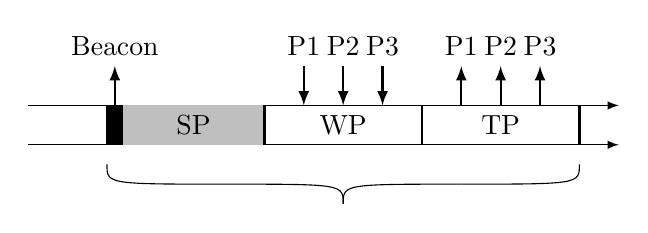
\begin{tikzpicture}[>=latex]
\draw[->] (-1cm,  0.25cm) -- +(7.5cm, 0);
\draw[->] (-1cm, -0.25cm) -- +(7.5cm, 0);
%beacon
\fill[black] (0cm, -0.25cm) rectangle +(0.2cm, 0.5cm);
\draw[->,thick] (0.1cm, 0.25cm) -- +(0, 0.5cm);
\draw (0.1cm, 1cm) node {Beacon};
%SP
\draw[thick] (0cm, -0.25cm) -- +(0, 0.5cm);
\fill[lightgray] (0.2cm, -0.25cm) rectangle +(1.8cm, 0.5cm);
\draw (1.1cm, 0) node {SP};
%WP
\draw[thick] (2cm, -0.25cm) -- +(0, 0.5cm);
\draw (3cm, 0) node {WP};
%TP
\draw[thick] (4cm, -0.25cm) -- +(0, 0.5cm);
\draw (5cm, 0) node {TP};
\draw[thick] (6cm, -0.25cm) -- +(0, 0.5cm);
%RX packets
\draw[->,thick] (2.5cm, 0.75cm) -- +(0, -0.5cm);
\draw (2.5cm, 1cm) node {P1};
\draw[->,thick] (3cm, 0.75cm) -- +(0, -0.5cm);
\draw (3cm, 1cm) node {P2};
\draw[->,thick] (3.5cm, 0.75cm) -- +(0, -0.5cm);
\draw (3.5cm, 1cm) node {P3};
%TX packets
\draw[->,thick] (4.5cm, 0.25cm) -- +(0, 0.5cm);
\draw (4.5cm, 1cm) node {P1};
\draw[->,thick] (5cm, 0.25cm) -- +(0, 0.5cm);
\draw (5cm, 1cm) node {P2};
\draw[->,thick] (5.5cm, 0.25cm) -- +(0, 0.5cm);
\draw (5.5cm, 1cm) node {P3};
%brace
\draw (0cm,-0.5cm)    .. controls +(0,-0.25cm) .. +(1.5cm,-0.25cm);
\draw (1.5cm,-0.75cm) .. controls +(1.5cm,0)   .. +(1.5cm,-0.25cm);
\draw (3cm,-1cm)      .. controls +(0,0.25cm)  .. +(1.5cm,0.25cm);
\draw (4.5cm,-0.75cm) .. controls +(1.5cm,0)   .. +(1.5cm,0.25cm);
\end{tikzpicture}
\caption{A typical S-CoSenS router duty cycle.}
\label{FigSCosensDutyCycle}
\end{figure}

We thus need to synchronize with enough precision different devices (that
can be based on different hardware platforms) on duty cycles whose periods
are dynamically calculated at runtime, with precision that needs to be
in the sub-millisecond range. This is where RIOT OS advanced real-time
features really shine, while the other comparable OSes are
for that purpose definitely lacking.

We have implemented S-CoSenS under RIOT, and made first tests by performing
simulations---with Cooja---of a 802.15.4 PAN (Personal Area Network)
constituted of a router, and ten motes acting as ``leaf nodes''.
The ten nodes regularly send data packets to the router, that retransmits
these data packets to a nearby ``sink'' device. Both the router and the ten
nodes use exclusively the S-CoSenS RDC/MAC protocol. This is summarized
in figure \ref{FigPANtest}.

\begin{figure}[!h]
\centering
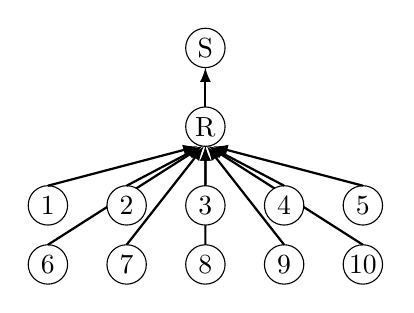
\begin{tikzpicture}[>=latex]
%sink
\draw (0, 1cm) circle (0.25cm); \draw (0, 1cm) node {S};
%router to sink link
\draw[->,thick] (0, 0.25cm) -- (0, 0.75cm);
%router
\draw (0, 0) circle (0.25cm); \draw (0, 0) node {R};
%leaf nodes (lower)
\foreach \x in {6,7,8,9,10}
{
  \fill[white] (\x * 1cm - 8cm, -1.75cm) circle (0.25cm);
  \draw (\x * 1cm - 8cm, -1.75cm) circle (0.25cm);
  \draw (\x * 1cm - 8cm, -1.75cm) node {\x};
  % link to router
  \draw[->,thick] (\x * 1cm - 8cm, -1.5cm)
                  -- (\x * 0.02cm - 0.16cm, -0.25cm);
}
%leaf nodes (upper)
\foreach \x in {1,2,3,4,5}
{
  \fill[white] (\x * 1cm - 3cm, -1cm) circle (0.25cm);
  \draw (\x * 1cm - 3cm, -1cm) circle (0.25cm);
  \draw (\x * 1cm - 3cm, -1cm) node {\x};
  % link to router
  \draw[->,thick] (\x * 1cm - 3cm, -0.75cm)
                  -- (\x * 0.05cm - 0.15cm, -0.25cm);
}
\end{tikzpicture}
\caption{Functional schema of our virtual test PAN.}
\label{FigPANtest}
\end{figure}

Our first tests clearly show an excellent synchronization between the
leaf nodes and the router, thanks to the precision offered by RIOT OS
event management system (especially the availability of many hardware
timers for direct use).

(Figure: copie \'ecran Cooja)

We were also able to collect data on duty cycle activity for both radio
transceivers and MCUs, they show RIOT allows for a very sparse use of
both transceiver and processing power:

(tableau)

While we weren't able to accurately quantize energy consumption yet, we can
reasonably think that lowering activity of MCU and radio transceiver will
significantly reduce the energy consumption of devices running RIOT OS.
This will be the subject of some of our future research works.

%%%%%%%%%%%%%%%%%%%%%%%%%%%%%%%%%%%%%%%%%%%%%%%%%%%%%%%%%%%%%%%%%%%%%%%%%%%%%

\section{\uppercase{Future Works and Conclusion}}

We plan, in a near future:

\begin{itemize}

\item to bring new contributions to the RIOT project: we are especially
      interested in the portability that the RIOT solution offers us;
      this OS is indeed actively ported on many devices based on powerful
      microcrontrollers based on ARM Cortex-M architecture (especially
      Cortex-M3 and Cortex-M4), and we intend to help in this porting
      effort, especially on high-end IoT motes we seek to use in our
      works (e.g.: as advanced FFD nodes with full network stack,
      or routers);

\item to use the power of this OS to further advance our work on MAC/RDC
      protocols; more precisely, we are implementing other innovative
      MAC/RDC protocols under RIOT, taking advantage of its high-precision
      real-time features to obtain excellent performance, optimal energy
      consumption, and out-of-the-box portability.

\end{itemize}

\bigskip

In conclusion, we can consider that we have actively contributed to the
development of a high-quality, full-featured, open-source software platform
for the domain of WSN, IoT, and even more largely of embedded computing.

Indeed, RIOT is a powerful real-time operating system, adapted to the
limitations of deeply embedded hardware microcontrollers, especially
in terms of minimization of memory footprint and energy consumption.
Nonetheless, it offers state-of-the-art techniques (preemptive
multitasking, tickless scheduler, optimal use of hardware timers)
that---we believe---makes it on par with the best OSes of the
emebedded and real-time world.

We are sincerely convinced that it will play an increasing role in
the WSN/IoT scene, and---hopefully---more generally in the embedded
computing world. We plan to both participate in its development,
and leverage its growth to further advance our work on networking
as far as possible.

%%%%%%%%%%%%%%%%%%%%%%%%%%%%%%%%%%%%%%%%%%%%%%%%%%%%%%%%%%%%%%%%%%%%%%%%%%%%%

\section*{\uppercase{Acknowledgements}}

The authors wish to thanks the members of the RIOT OS project,
especially the core development team, for their kind welcome
in the RIOT project, and their enhtusiasm and friendliness
toward us. And, of course, for designing and publishing
this awesome software platform.


\vfill
\bibliographystyle{apalike}
{\small
\bibliography{sensornets2015}}


\end{document}
